% Chapter Template

\chapter{STATE-OF-THE-ART ABOUT VMI} % Main chapter title

\label{Chapter2} % Change X to a consecutive number; for referencing this chapter elsewhere, use \ref{Chapter2}

\lhead{Chapter 2. \emph{STATE-OF-THE-ART ABOUT VMI}} % Change X to a consecutive number; this is for the header on each page - perhaps a shortened title

In this section, we firstly present some important background conceptions and terminology about VMI technology, then look through the evolution of VMI, finally analyze and synthetize some typical VMI applications to get a panorama about this emerging technology.  

%----------------------------------------------------------------------------------------
%	SECTION 1
%----------------------------------------------------------------------------------------

\section{SEMANTIC GAP \citep{Reference26}}

The fundamental challenge faced by all VMI applications is to bridge the semantic gap. Theoretically, the hypervisor is capable of retrieving all low-level binary data (for example memory page, network traffic, etc.) from guests which it manages. These binary data contains almost all running states of VM. However, without more extra semantic knowledge about guest OS or hardware architecture, hypervisor could not extract high-level information about running states of guests and thus is not able to react to guests’ activities. This lack of extra semantic knowledge is called semantic gap.  


\section{VMI-RELATED TERMINOLOGY}

\subsection{Semantically awareness VS semantically unawareness}

According to semantic awareness, all VMI applications fall into two categories: semantically awareness and semantically unawareness[3], An application characterized as semantic aware means that it conducts monitoring task by extracting information related to guest OS (for example, guest OS kernel data structure, guest memory lay out, etc.). On the contrary, semantic unawareness VMI application seeks to infer other information than OS-related semantic information, a typical example for this kind of application is Antfarm  \citep{Reference4}. Obviously, the semantically unaware applications are less powerful compared to semantically aware VMI application in terms of account of running state. However, usually, the former is more robust against a majority of circumstance technique. Thus in practice, it’s difficult and usefulness to judge which kind of approach is much better. It’s better to combine respective advantages of these two approaches.

\subsection{Derivative pattern VS Delivery pattern}

The taxonomy of VMI application could be talked in another perspective. On the basis of the manner by which semantic information is gathered by hypervisor, all VMI applications could be implemented in three patterns: in-band pattern, out-of-band pattern and derivative pattern [5]. In-band pattern describes the case where an internal agent in VM gather and delivery information to hypervisor. Strictly speaking, In-band pattern is not a real VMI method, thus it is not an investigation focus. Out-of-band pattern is the most commonly used method to bridge the semantic gap. Its main idea lies in that hypervisor obtains in advance some semantic knowledge, such as System symbol file for Linux guest, to extract subsequently more running states of VM. VMI in out-of-band is the most active research domain compared to the other two patterns. The last pattern is derivative pattern whose principle is to extract and infer running states information about guest from semantic knowledge of hardware architecture. It seems that this pattern is ideal for implementing VMI applications. However, derivative pattern could be used in limited cases. To what extent this limitation exists is further explored in chapter 6 by Pfoh [7]. In addition, the investigation about derivative pattern is much fewer than that of out-of-band. Nitro, Antfarm and Lycosid [4, 8, 9] are three typical VMI applications in this domain.

\subsection{Reutilization pattern}

This is a term I personally add to cover those VMI applications whose principal philosophy is reutilization of binary code or execution context \citep{Reference27, Reference28}. Compared with other patterns (delivery or derivative pattern), it is a big step in automating of generation introspection tool.


\section{VMI TECHNOLOGY EVOLUTION}

The prevalence of virtualization technologies gives new opportunities for VMI, at the level of hypervisor, to inspect and analyze both the user level program and OS kernel states outside the virtual machine itself. However, the key challenge in VMI is to bridge the semantic gap. Many approaches are proposed to address this problem over the past decade. This section is devoted to talk about the evolution of VMI in terms of implementation philosophy and their respective point of innovation and limitation.
The first attempt [1] of bridging the semantic gap is to leverage the Linux crash utility (a kernel dump analysis tool), but this solution requires the kernel to be recompiled with the debugging symbols. Therefore, limitation of this approach is rather obvious: not convenient and is uniquely applied to open-source OS such as Linux. The significance of this solution resides in that it for the first time validates the practicability of VMI technologies. Much more efforts are still required to make VMI a practical solution in cloud environment.

Given that the view of hypervisor for guest is just raw data (0/1 bit series) of memory and vCPU registers, it is rather intuitive and logic to overcome the semantic gap by leveraging manual kernel data traversal approach. Some research efforts [2] are representative examples following this approach. Its idea is to locate, traverse, and interpret known data structure of the in-guest memory. While this solution has been widely adopted between 2003 and 2011, many of them rely on a manual effort or compiler-assistant approach to locate the in-guest kernel data and develop the in-guest semantic-equivalent code for the introspection. This approach is indeed a significant step in the road to remedy the semantic gap. However, VMI introspection applications based on this approach suffer from frequent changes due to the constant update or patch of kernel. More importantly, this approach requires an intimate knowledge about OS kernel or reverse engineering. Furthermore, it may also introduce vulnerabilities for attackers to evade these hand-built introspection tools.

To relieve the painful process of adapting introspection utilities caused by the changes to OS kernel, some researchers [4, 7] tried to retrieve meaning high-level information from hardware architecture such as Intel X86 architecture. Although this method is guest-OS agnostic, the high-level information could be revealed is rather limited. Thus this approach is also far from practical for cloud providers. 

All existing solutions to narrow semantic gap before 2011 mostly rely on manual efforts and reverse engineering skills, which pose problems to deploy VMI in cloud environment. Suppose we have already a perfect approach to bridge the semantic gap, we still have to develop some guest OS management utilities from scratch to mimic the similar in-guest inspection programs (ps/netstat,etc.). Based on this observation, people think of reusing the legacy binary code instead of developing extra new vulnerability-prone programs. Under the guide of this philosophy, Dolan-Gavitt et al [27] presented VIRTUOSO, which made a significant attempt in this perspective. VIRTUOSO made a first step showing that we could actually reuse the legacy binary code to automatically create VMI tools with the assistance from a human expert. Its key idea is to first train each in-VM program (e.g., ps) and then translate the trained traces (essentially slices) into an independent introspection program running at the hypervisor layer. However, due to the nature of dynamic analysis, VIRTUOSO is only able to reproduce introspection code that has been executed and trained. Meanwhile, it is not fully automated and requires the intervention from a human expert.

Drawing inspiration from VIRTUOSO, VMST [28] shows a dual-VM based online kernel data redirection approach that addresses the limitations from the training existing in VIRTUOSO. Unlike VIRTUOSO, VMST reuses the execution context of an inspection process in a trusted VM: When a kernel instruction accesses the kernel data of introspection interest, it redirects the data from the guest VM to the trusted VM.

Built atop of VMST, the same research team proposed EXTERIOR [29], which is a novel dual-VM based external shell for trusted, native, out-of-VM program execution for guest-OS administration including introspection, configuration and recovery. Unlike pre-existing VMI techniques, EXTERIOR for the first time enables an out-of-VM shell with a guest-OS writable and executable capability. Its key idea is to leverage an identical trusted kernel with the guest-OS to create the necessary environment for a running process in a SVM (trusted VM), and transparently and dynamically redirect and update the memory at the VMM level to a GVM, thereby achieving the same effect in terms of kernel state updates of running a program inside a guest-OS. Traditionally, shells are designed atop an OS kernel, EXTERIOR demonstrates that a shell could also be designed below an OS. Thus, one important significance of EXTERIRO lies in that it presents a new program execution model on top of virtualization. While EXTERIOR has made an early attempt of building a hypervisor layer shell, it has a lot of constraints and is far from practical: Firstly, it has to first perform the guest OS fingerprinting [30] and then use the exact same version of the guest OS running in a SVM to introspect the kernel state of a GVM. Second, it can suffer from various failures and shortfalls when an introspection related system call uses kernel synchronization primitives [28].Third, it is built atop a binary code translation based VM which often has 10-40X performance slowdown. 

HyperShell [31] has drawn inspirations from Process Implanting [32] and extended EXTERIOR. To overcome the semantic gap challenge, HyperShell introduces a reverse system call(R-syscall in short) abstraction. This abstraction serves as the interface in a reverse direction from a layer up and it is also transparent to legacy software (e.g. ps/lsmod/netstat/ls/cp). This design allows a large number of legacy in-guest management utilities executing directly at hypervisor level with no modification. HyperShell still remains some limitations: First, it needs a log record at the hypervisor layer for each activity executed in HyperShell (Security concern). Second HyperShell requires a trusted guest OS kernel and init process thus could not be used for security critical applications. Third, current prototype requires both OS running in the host OS and the GVM to have compatible syscall. Finally, static linked native utilities cannot be executed in HyperShell.

Briefly speaking, the semantic gap problem is still a difficult, open research problem today. More advances and innovations are required to make VMI technology applicable in production environment.



\section{REPRESENTIVE VMI APPLICATION}

As one of internship’s objectives, plenty of VMI applications or development frameworks are analyzed and synthesized. It is at the same time an interesting complement for above section in another perspective. Because of space constraints, it’s impossible to collect and analyze all existing VMI applications. Here, we just pick up those regarded as milestone and having reference value in this domain.

\subsection{Delivery Pattern VMI Application}

VMI theory is initially proposed by Garnkel and Rosenblum  \citep{Reference1} in 2003. As a proof-of-concept prototype of their theory, Lirewire  \citep{Reference1} is the first VMI application whose objective is to deploy a firewall on hypervisor level. The significance of Lirewire is to prove the feasibility of VMI from within hypervisor. However, it could not give us technical inspiration, thus here its implementation will not be talked about.

VIX  \citep{Reference10}, which stands for Virtual Introspection for Xen, is a tool suite on the basis of the out-of-band delivery pattern for forensic analysis. This system uses delivered knowledge about the guest OS in order to implement common UNIX tools such as ps, lsmod and netstat. Although this tool suite is close to what we want to implement, it unfortunately does not support KVM hypervisor and its code is not accessible.

RTKDSM  \citep{Reference3}, for Real-Time Kernel Data Structure Monitoring, leverages the rich OS analysis capabilities of Volatility  \citep{Reference13} to significantly simplify and automate analysis of VM execution states. Its implementation is under Xen platform, inspiration that it could give us is the use of Volatility who provides vast kernel data structure knowledge to remove the burden of bridging semantic gaps from VMI application developers.

Other systems such as HookSafe, NICKLE are all presented by Pfoh in his work  \citep{Reference7}. They both rely on out-of-band to mitigate the semantic gap to monitor or protect the integrity of kernel code. As their close source nature, they could not give us more help. All mentioned VMI applications are summarized in the following table. It is supposed to note that this is not an exhaustive table and there all still many others VMI applications in this filed.

\begin{figure}[htbp]
	\centering
		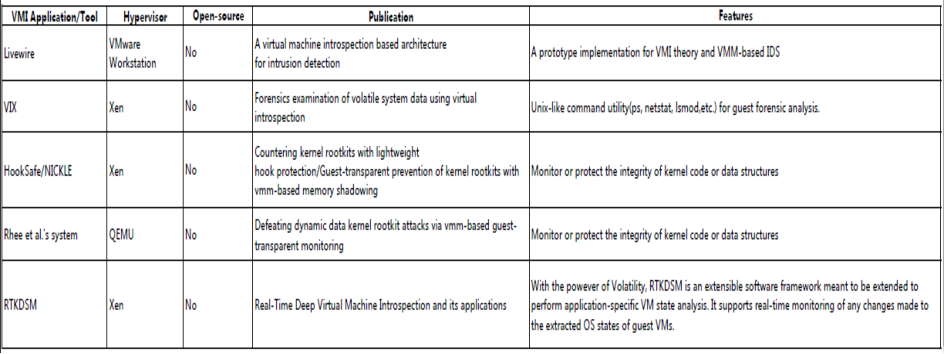
\includegraphics{Figures/Figure1.pdf}
		\rule{35em}{0.5pt}
	\caption[Out-of-Band pattern VMI applications]{Out-of-Band pattern VMI applications}
	\label{fig:Out-of-Band pattern VMI applications}
\end{figure}


\subsection{Derivative Pattern VMI APPLICATION}
Then we talk about some VMI applications based on derivative pattern. Manitou system use x86’s paging mechanism to perform integrity checks before code execution. From this work, we find paging mechanism is an important filed to explore to leverage derivative method. Antfarm is another typical example for derivative pattern. It is specially designed to monitor the VM’s memory management unit (MMU). From that, it could construct the virtual-to-physical memory mapping and retrieve all running processes identified by a CR3 register value in guest. Lycosid allows detecting and identifying all those hidden processes in guest. It first retrieves two different level process lists (cross-view validation) in guest by respectively using Antfarm and guest built-in utility (for example “ps” command in Linux/Unix world.). If number of processes contained in these two different lists is not pertinent, Lycosid then infer the presence of some hidden processes and deduce those processes hidden by some statistical methods. Antfarm and Lycosid are both implemented in Xen platform and we have no access to its source code. However, these two systems show a typical situation where we could apply derivative pattern. From these two applications, we also get to know that derivative pattern is really useful for security purpose, due to the fact that even though Lycosid is not familiar with the malicious process (PID, process name, etc.), it could interfere those dangerous activities.

Nitro, as far as I know, is the most recent derivate-pattern VMI application, whose objective is to trap system call events according to user-defined filter rule. For example, Nitro could be used as a technical building block retrieving all system calls for malware analysis. Due to its derivative pattern and open-source nature, Nitro is the focus of my investigation. Based on its functionality to access vCPU’s registers and system call trap, we intend to add network traffic monitoring functionality to Nitro and implement network monitoring on process granularity. However, Nitro is just under maintenance of Pfoh and has no updates since almost six months, even though it is an open-source project. Thus, there is not enough documentation about its utilization and it needs some enhancements besides its provided basic functionality. Further introduction about Nitro are in the following part. All these derivative pattern VMI applications are summarized in the following table.

\begin{figure}[htbp]
	\centering
		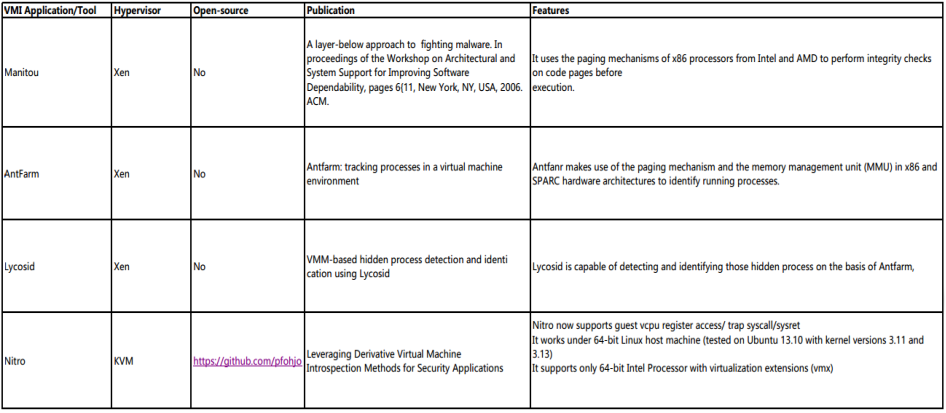
\includegraphics{Figures/Figure2.pdf}
		\rule{35em}{0.5pt}
	\caption[Derivative pattern VMI applications]{Derivative pattern VMI applications}
	\label{fig:Derivative pattern VMI applications}
\end{figure}



\section{VMI RELATED TOOLS}

Besides those mentioned VMI applications, we then talk about some interesting VMI Tools. These tools themselves are not VMI applications aiming for certain security problems. Instead they may be in form of C library providing general VMI functionalities or forensic analysis frameworks to help bridge the semantic gap.


\subsection{LibVMI/XenAccess  \citep{Reference10,Reference11}}

LibVMI is an introspection library focused on reading and writing memory from running virtual machines. For convenience, LibVMI also provides functions for accessing CPU registers, pausing and unpausing a VM, printing binary data, and more. LibVMI is designed to work across multiple virtualization platforms. LibVMI currently supports VMs running in either Xen or KVM. LibVMI also supports reading physical memory snapshots when saved as a file.

XenAccess is predecessor of LibVMI but is focused exclusively on Xen. LibVMI is designed to work across a variety of virtualization platforms including Xen and KVM. LibVMI provides a more intuitive API and therefore is more advised compared to XenAccess. Please refer to the following link for more information: https://code.google.com/p/vmitools/. 

\subsection{Volatility  \citep{Reference13}}

The Volatility is an excellent open-source forensic analysis framework implemented in Python. It presents the advantage of bridging the semantic gap regardless of the system being monitored. Volatility has a wide range memory dump support, from Windows to Linux, from Mac OS to Android. Also, there exist plenty of tutorials about this framework. Thus, recent years have witnessed increasing adoption of Volatility in VMI application development, for example RTKDSM system. For more information, refer to this link: https://code.google.com/p/volatility/.

\subsection{Insight-VMI  \citep{Reference14,Reference15}}

Similar to Volatility, Insight-VMI is another open-source forensic analysis framework written in C++. Compared to Volatility, it additionally provides an interactive shell for manual analysis of kernel objects and a JavaScript engine for automated analysis of repeating or complex tasks, but it now supports only Linux memory analysis. In addition, Insight-VMI and Nitro are both developed and maintained by the same study team at the Technische Universität München in Germany. Detailed information is available in: https://code.google.com/p/insight-vmi/.

\begin{figure}[htbp]
	\centering
		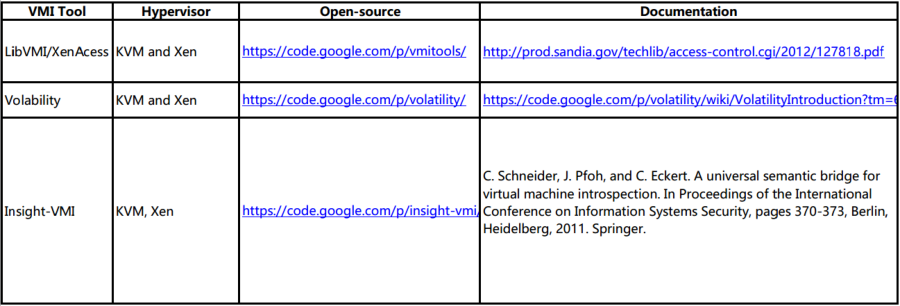
\includegraphics{Figures/Figure3.pdf}
		\rule{35em}{0.5pt}
	\caption[VMI Tool manifest]{VMI Tool manifest}
	\label{fig:VMI Tool manifest}
\end{figure}



